\documentclass[twocolumn]{article}
\usepackage{caption}
\usepackage[utf8]{inputenc}
\usepackage{amsmath}
\usepackage[margin=1in]{geometry}
\usepackage{changepage}
\usepackage{titling}
\usepackage{ragged2e}
\usepackage{abstract}
\usepackage{enumitem}
\usepackage{graphicx}
\usepackage{hyperref}
\renewcommand{\thesection}{\Roman{section}}
\renewcommand{\thesubsection}{(\roman{subsection})}
\setlength{\columnsep}{1cm}
\setlength\parindent{5pt}
\DeclareMathOperator{\arccosh}{arccosh}

\begin{document}
\twocolumn[
\begin{@twocolumnfalse}
\title{\Large{\textbf{AC and DC Hall Effect experiment on a 300$\mu m$ 
Si doped wafer}}}
\author{Herbert D. Ludowieg}
\setlength{\droptitle}{-0.65in}
\maketitle
\begin{onecolabstract}
\justify
The Hall Effect is a phenomena of solid materials that has been in use since 
the turn of the century. In this experiment we used the AC and DC hall effect 
to see the properties of a Si doped semiconductor sample including: the type 
of semiconductor, carrier mobility and density and the resistivity of the 
sample. It was determined the sample was an n-type emiconductor, with a 
temperature dependent carrier density with values: 3.08$x10^{20}$ 
$\pm$ 0.09$x10^{20}$ at 80K, 3.1$x10^{20}$ $\pm$ 0.3$x10^{20}$ at 100K, 
3.06$x10^{20}$ $\pm$ 0.07$x10^{20}$ at 120K, 2.83$x10^{20}$ $\pm$ 
0.04$x10^{20}$ at 140K, 2.8$x10^{20}$ $\pm$ 0.1$x10^{20}$ at 160K, 
3.5$x10^{20}$ $\pm$ 0.1$x10^{20}$ at 180K, 3.12$x10^{20}$ $\pm$ 0.07$x10^{20}$ 
at 200K, 3.8$x10^{20}$ $\pm$ 0.2$x10^{20}$ at 220K, 3.8$x10^{20}$ $\pm$ 
0.2$x10^{20}$ at 240K and 3.9$x10^{20}$ $\pm$ 0.2$x10^{20}$ at 260K. With 
temperature dependent values of: 1.44$x10^{-2}$              
$\pm$ 0.05$x10^{-2}$ at 80K, 1.5$x10^{-2}$ $\pm$ 0.1$x10^{-2}$ at 100K, 
1.49$x10^{-2}$ $\pm$ 0.03$x10^{-2}$ at 120K, 1.63$x10^{-2}$ $\pm$ 
0.03$x10^{-2}$ at 140K, 1.7$x10^{-2}$ $\pm$ 0.07$x10^{-2}$ at 160K, 
1.47$x10^{-2}$ $\pm$ 0.06$x10^{-2}$ at 180K, 1.77$x10^{-2}$ $\pm$ 
0.04$x10^{-2}$ at 200K, 1.57$x10^{-2}$ $\pm$ 0.07$x10^{-2}$ at 220K, 
1.68$x10^{-2}$ $\pm$ 0.09$x10^{-2}$ at 240K and 1.69$x10^{-2}$ $\pm$ 
0.07$x10^{-2}$ at 260K.\\ \\
\end{onecolabstract}
\end{@twocolumnfalse}
]
%\begin{multicols}{2}
\justify
\section{Introduction}
The hall Effect was discovered by Edwin H. Hall in 1879, who at the time was 
studying under Rowland at Johns Hopkins University. During those days no one knew of 
the electron and by extension how it was that conduction actually happened. 
Due to this it took almost 50 years until the Hall Effect was fully understood 
with the formulation of quantum mechanics. The results that were gotten from 
the experiment were generally not very well understood \cite{ref:1}.
\\
However, when quantum mechanics was formulated and the Hall Effect became fully 
understood it began to be employed in the study of semiconductors. It was here 
that it fullfilled its promise in the study of the concentration and sign of 
charge carriers \cite{ref:1}. Both of which are to be found in this experiment. 
\\
There are four different types of materials: insulators and superconductors, 
semiconductors and conductors. The difference between all of these are the 
resistivity and conductivity values for them. Insulators and superconductors 
behave in a very similar fashion in that they allow almost no current to pass 
through them, they have near infinite resistivities and near zero conductivity 
values. Conductors are the polar opposite of them having very low resistivity 
values and extremely high conductivity. Semiconductors are the middle ground 
where the two meet having finite resistivity and conductivity values.
\\
Semiconductors are an integral 
part in our daily lives since they have been in wide use in electronics such 
as: computers, cell phones and LED bulbs. The Hall Effect has given a far 
reaching insight into how and why it is that the properties listed above 
display such distinct behaviors.
\\
For the experiment a large electromagnet with a magnetic field range of 0 T to 
0.6678 T was used to create a homogenous strong magnetic field. To receive the 
signals a lock-in amplifier was used for the AC Hall Voltage measurements and a 
simple multi-meter was used to measure the DC Hall Voltage measurements. The 
temperature of the sample could also be controlled via a PID temperature 
controller that allowed to heat up the sample and it was cooled down through 
the use of Liquid Nitrogen (LN). The sample was housed in a cryostat chamber 
containing a very dilute Helium gas concentration to be a thermal contact 
between the inner chamber and the LN.
\\
The sample was a Silicon doped semiconductor which we put at cryogenic 
temperatures and in a high intensity magnetic field to perform the measurements.
\section{Theory}
%\begin{wrapfigure}{l}{0pt}
\begin{figure*}
\begin{minipage}[t]{0.46\textwidth}
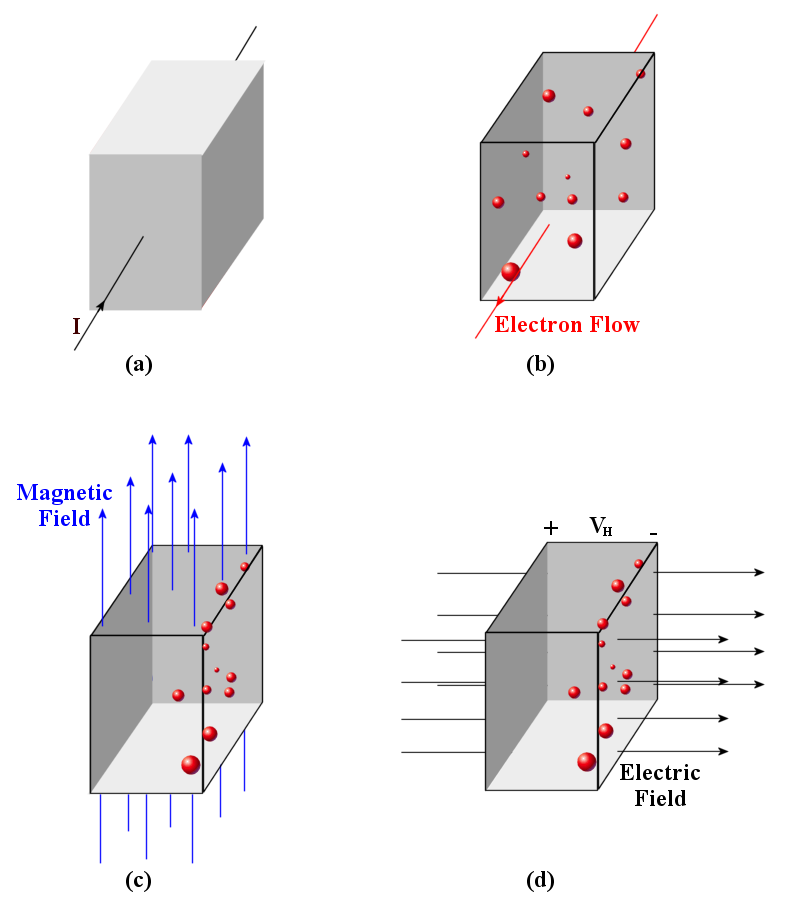
\includegraphics[width=\linewidth,height=\linewidth]{shift-electrons.png}
\caption{a). Representation of the general setup wiyh the sample and a wire 
providing current through the sample. b). A general representation of the flow 
of electrons in the sample. c). The general shift in the position of the 
electrons as they pass through a magnetic field. d). Electric field that is 
produced when the electrons distribute themselves in such a manner 
\cite{ref:2}.}
\label{fig:1}
\end{minipage}
\hfill
\begin{minipage}[t]{0.46\textwidth}
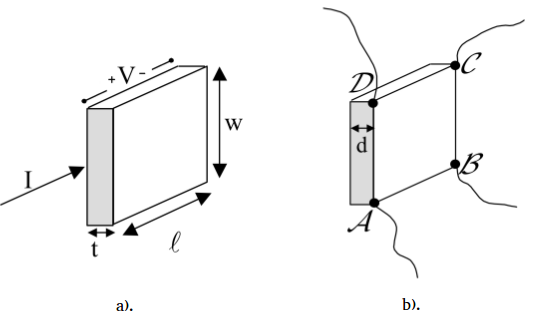
\includegraphics[width=\linewidth]{contacts-dim.png}
\caption{a). Current passing through a sample of dimension l,w,t. b). Sample of
depth d with four contacts placed on the corners of the sample.}
%\cite{ref:3}
\label{fig:2}
\end{minipage}
\end{figure*}
%\end{wrapfigure}
From electricity and magnetism we know that charged particles passing through 
a magnetic field display the following force relation,
\begin{equation}
\label{eqn:1}
\vec{F}=q(\vec{E}+\vec{v}\times\vec{B})
\end{equation}
Where, q is the charge of the particle, $\vec{E}$ is the electric field 
in the space of the particle, $\vec{v}$ is its velocity and $\vec{B}$ is the 
magnetic field. Usually, we can consider the contribution of the electric field 
to the force to be zero so we can write equation \ref{eqn:1} as,
\begin{equation}
\label{eqn:2}
\vec{F}=q\vec{v}\times\vec{B}
\end{equation}
So that is to say that the charge carriers will receive a force that is 
perpendicular to their motion and as a cause will begin to curve. If we now 
think about a solid material through which we pass some current it would look 
like figure \ref{fig:1}b. Where the electrons are free to move through the 
entire sample and have nothing directing their movement other than the electric 
current that is passing through the sample. For a pictorial representation of 
what happend when we apply a strong magnetic field perpendicular to the sample 
refer to figures \ref{fig:1}c,d. This makes sense with equation \ref{eqn:2} and 
what we generally know of charged particles passing through a perpendicular 
magnetic field. Looking at figure \ref{fig:1}d the reason why it does in fact 
produce an electric field inside of the sample is due to the electrons that 
have curved to a side of the sample and since they can't conduct very easily 
through the a air they accumulate at the boundary of the sample toward which 
they curve creating a gradient of electrons and lack of electrons (positive 
charge) which gives rise to a potential difference through the sample and 
therefore an electric field through the sample.
\\
This perpendicular magnetic field can be calculated with equation \ref{eqn:3}.
\begin{equation}
\vec{E}_t = \frac{-\vec{J}\times\vec{B}}{nq}
\cite{ref:1}
\label{eqn:3}
\end{equation}
Where, $\vec{J}$ is the current density, $\vec{B}$ is the magnetic field 
passing through the sample,n is the number carriers and q is the charge of the 
carriers.
\\
Equation \ref{eqn:3} is mainly useful were qe to know all of the 
parameters we need which, for this experiment, we need to find. So we take a 
different approach in our equation derivations starting with how to calculate 
the resistivity of a semiconductor sample.
\\
When we have a sample with a current passing through it of certain current 
density, j, We can show that the electric field is related in the following way,
\begin{equation}
\vec{E} = \rho\vec{j}
\cite{ref:3}
\label{eqn:4}
\end{equation}
Where, $\rho$ is the resistivity of the sample. By multiplying both sides of 
equation \ref{eqn:3} by the length of the sample, l, we can get a relation 
between the voltage and the resistivity.
\begin{equation}
V = \rho\frac{l}{tw} I 
\cite{ref:3}
\label{eqn:5}
\end{equation}
Where, l,t,w are the dimensions shown of figure \ref{fig:2}b and I is the 
total current through the sample. By then applying Ohm's law, V=IR, we can get 
to the relation of resistance with resistivity.
\begin{equation}
R = \rho\frac{l}{wt} = R_s\frac{l}{w}
\cite{ref:3}
\label{eqn:6}
\end{equation}
Where, $R_s = \rho/t$. $R_s$ is the sheet resistance of the sample and it is 
only dependent on the thickness of the sample as per the equation. Notice that 
if the sample is perfectly square, l=w, $R_s = R$ \cite{ref:3}. By performing a 
two contact resistivity measurement we can receive values for the resistivity 
of the sample. However, as it will be more apparent later these values that we 
get do have a certain amount of error and a more accurate method can be 
employed. This method is the va der Pauw method which was developed in 1958 by 
Leo J. van der Pauw.
\\
To use this method the following conditions must be met \cite{ref:4}.
\begin{enumerate}[label=\alph*]
\item The contacts are at the circumference of the sample.
\item The contacts are sufficiently small.
\item The sample is homogeneous in thickness.
\item The surface of the sample is singly connected,i.e.,the sample does not 
have isolated holes.
\end{enumerate}
Now, the first condition assumes that the sample is a disc, but this method can 
work for any shape like a square. The derivation of the method can be found in 
\cite{ref:3}
Now, the first condition assumes that the sample is a disc, but this method can 
work for any shape like a square. The derivation of the method can be found in 
\cite{ref:3}. In figure \ref{fig:2}b we see that the contacts are placed in the 
corners. They do not have to necessarily be on the corners. They can be 
anywhere along the edge of the sample. According to van der Pauw's paper the 
resistivity of a sample using the four contact method can be calculated with 
the following equation.
\begin{equation}
\rho = \frac{\pi d}{\ln{2}}\frac{R_{AB,CD}+R_{BC,DA}}{2}f\left(\frac{R_{AB,CD}}{R_{BC,DA}}\right)
\cite{ref:4}
\label{eqn:7}
\end{equation}
\begin{figure*}
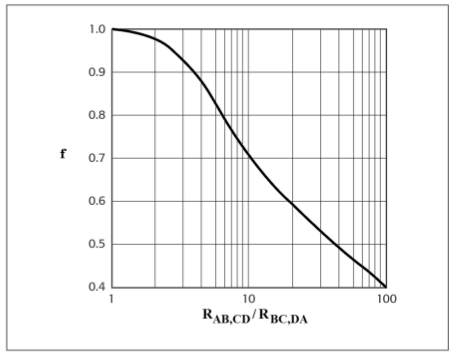
\includegraphics[width=\textwidth,height=3.5in]{f-function.png}
\caption{Plot of the f function from equation \ref{eqn:6} \cite{ref:3}.}
\label{fig:3}
\end{figure*}
Where, d is the thickness of the sample (t in the case of fig. \ref{fig:2}b), 
$R_{AB,CD}$ and $R_{BC,AD}$ represent current passing through the point and 
making the voltage measurement respectively. That is to say they are along the 
perpendicular current directions as can be inferred from figure \ref{fig:2}b. 
The function f is a function that behaves in 
similar fashion to that which is shown on figure \ref{fig:3}. Where it only 
satisfies the relation.
\begin{equation}
\frac{R_{AB,CD}-R_{BC,DA}}{R_{AB,CD}+R_{BC,DA}} = f\arccosh{\frac{\exp{(\ln{(2/f)})}}{2}}
\cite{ref:4}
\label{eqn:8}
\end{equation}
Which can only be solved numerically to solve for f. Van der Pauw does provide 
another equation to approximate f where the ratio of $R_{AB,CD}/R_{BC,DA}$ are 
almost equal.
\begin{equation}
\begin{split}
f \approx 1-\left(\frac{R_{AB,CD}-R_{BC,DA}}{R_{AB,CD}+R_{BC,DA}}\right)^2\frac{\ln{2}}{2}- \\
\left(\frac{R_{AB,CD}-R_{BC,DA}}{R_{AB,CD}+R_{BC,DA}}\right)^4\left\{\frac{(ln{2})^2}{4}-\frac{(\ln{2})^2}{12}\right\}
\cite{ref:4}
\label{eqn:9}
\end{split}
\end{equation}
There is another method that can be used in which we use a table which is 
provided to us. However, to reduce errors from approximating to the second 
decimal point the f value is calculated for every ratio and was compared to the 
given f values. They agreed to the second decimal and was believed to be a 
better approximation than those given in the table.
\\
In general, we can represent the resistivity and conductivity of a sample of 
comparable size as a tensor meaning that the electric field and the current 
density may not necessarily be parallel to one another. Such matrices are the 
following.
\begin{equation*}
\begin{align*}
\rho &= 
\begin{bmatrix}
\rho_{xx}&\rho_{xy} \\
-\rho_{xy}&\rho_{yy}
\end{bmatrix}
\\
\sigma &= 
\begin{bmatrix}
\sigma_{xx}&\sigma_{xy} \\
-\sigma_{xy}&\sigma_{yy}
\end{bmatrix}
\end{align*}
\end{equation*}
Where, the x and y subscripts represent the sheet coordinate directions of the 
sample ignoring the z.
\\
Back in equation \ref{eqn:3} we showed the relation between the current density 
and the magnetic field to find the electric field that is produced by the Hall 
Effect. Here, a different form of it will be shown using vectors and tensors.
\begin{equation}
\begin{bmatrix}
E_{x}\\E_{y}
\end{bmatrix}
=
\begin{bmatrix}
\rho_{xx}&\rho_{xy} \\ 
-\rho_{xy}&\rho_{yy}
\end{bmatrix}
\begin{bmatrix}
j_x \\ 0
\end{bmatrix}
\cite{ref:3}
\label{eqn:10}
\end{equation}
Where, $j_y = 0$ since there is no input current along the y direction of the 
sample only along the x direction. When equation \ref{eqn:10} is solved for the 
electric field components we can get the following equations.
\begin{equation}
\begin{align*}
E_x &= \rho_{xx}j_x\\
E_y &= -\rho_{xy}j_x
\cite{ref:3}
\label{eqn:11}
\end{align*}
\end{equation}
Where, if we transform equation \ref{eqn:11} as we did with equation 
\ref{eqn:4} we get a 
relation between $V_Hall$ and the xy resistance of the sample. Keep in mind 
that it is the Hall voltage as the field in the y direction is a direct cause 
of the magnetic filed that is along the z direction.
\begin{equation}
V_{Hall} = R_{xy}I
\cite{ref:3}
\label{eqn:12}
\end{equation}
Where, $R_{xy}$ is given by the equation.
\begin{equation}
R_{xy} = \frac{R_H}{t}B
\cite{ref:3}
\label{eqn:12}
\end{equation}
Where, $R_H$ is the Hall constant which depends on the carrier density and the 
charge of the carriers as shown.
\begin{equation}
R_{H} = \frac{1}{nq}
\cite{ref:3}
\label{eqn:13}
\end{equation}
Where, n is the number of carriers per unit volume and q is the charge of such 
carriers. Since, n is a integer value the sign of the Hall constant solely 
depends on the charge of the carriers. So, if the Hall constant is negative the 
charge carriers of the sample will be electrons and in the case of a positive 
value it will be holes (positive charge areas). In semiconductors this helps to 
identify what type of doping is used. If the semiconductor is n-type there is 
an excess of electrons where if it is p-type there is an excess of positively 
charged holes. Must be careful to not say protons as they do not flow when 
conducting electricity.
\\
By combining equations \ref{eqn:12} and \ref{eqn:12} we can make the following 
relationship between the Hall constant and the magnetic field.
\begin{equation}
R_{H} = \frac{V_{Hall}}{B}\frac{t}{I}
\cite{ref:3}
\label{eqn:14}
\end{equation}
Where, we can also re-write the equation to make the relationship between the 
magnetic field and the carrier density in a sample.
\begin{equation}
n = \frac{B}{V_{Hall}}\frac{I}{qt}
\label{eqn:15}
\end{equation}
\begin{figure*}
\begin{minipage}[t]{0.46\textwidth}
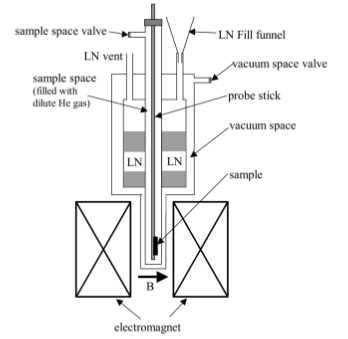
\includegraphics[width=\linewidth]{cryostat.png}
\caption{A general diagram of the cryostat that is to be used. There are three 
chambers in the cryostat \cite{ref:3}.}
\label{fig:4}
\end{minipage}
\hfill
\begin{minipage}[t]{0.46\textwidth}
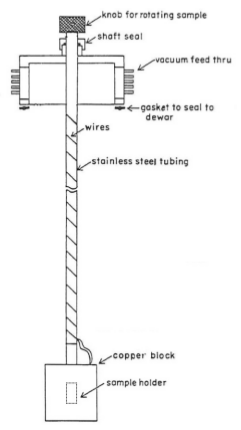
\includegraphics[width=1.5in]{sample-probe.png}
\caption{Schematic of the sample probe \cite{ref:3}.}
\label{fig:5}
\end{minipage}
\end{figure*}
Carrier mobility is defined as the ability of a charge carrier to pass through 
a sample material. The carrier mobility can be defined as the ratio between the 
drift velocity and the applied electric field. Which by transforming into the 
components of the electric field we can represent the carrier mobility as a 
function of the carrier density or the Hall constant.
\begin{equation}
\begin{align*}
\mu &= \frac{1}{\rho nq} \\
    &= \frac{R_H}{\rho} \\
    &= \frac{V_{Hall}}{B}\frac{t}{\rho q}
\cite{ref:3}
\label{eqn:16}
\end{align*}
\end{equation}
\section{Experimental Set-Up}
\begin{figure*}
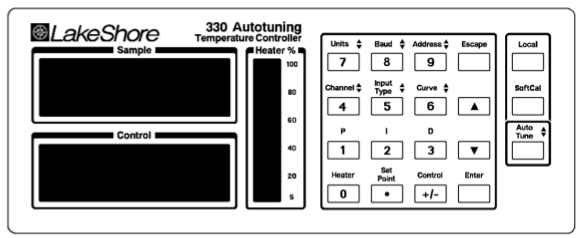
\includegraphics[width=\textwidth]{temperature-cont.png}
\caption{Front panel of the temperature controller with the labeled components
\cite{ref:3}.}
\label{fig:6}
\end{figure*}
For this experiment a combination of equipment was used to make the 
measurements including a cryostat which housed the sample probe containing the 
sample, a temperature controller, a lock-in amplifier, a DC source, a vacuum 
pump and an electromagnet.
\subsection{Cryostat}
Since, it is necessary to make low temperature measurements in this experiment 
a three chamber cryostat is to be used. Where, the chambers are labeled on 
figure \ref{fig:4}. The inner and outer chambers must be at a near vacuum 
which can be 
achieved with the provided vacuum pump. \textbf{NEVER add liquid nitrogen until 
the air in the cryostat is evacuated}. Not doing so could result in the air 
moisture condensing inside the cryostat when the liquid nitrogen is added. The 
inner chamber should be vacummed twice once to remove most of the air in the 
chamber and a second time by putting Helium gas in the chamber and proceeding 
to them vacuum the Helium gas out of the chamber. This ensures that most if 
not all of the air has been taken out of the chamber and only very dilute He 
gas is left in the chamber. The outer chamber should be vacuumed for 5 minutes 
as it is a much larger volume than the inner chamber. Should the air in the 
cryostat freeze the sample or the entire cryostat could be damaged \cite{ref:3}.
\\
Once this is done the liquid nitrogen can be added into the cryostat by use of 
the funnel. The cryostat has a max capacity of approximately 5 liters of 
liquid. Be careful when puring the liquid nitrogen as it will sputter when it 
comes into contact with the funnel. \textbf{Always wear the safety equipment 
provided including: cryo-gloves, goggles and the lab coat} \cite{ref:3}.
\subsection{Sample probe}
The sample to be tested is mounted on a sample probe that will be placed in the 
cryostat by the instructor and won't need to be taken out. If there is ever a 
problem and it does need to be taken out of the cryostat the entire cryostat 
must reach room temperature before doing anything as breaking the seal in the 
inner chamber could damage the cryostat. The sample holder is shown on figure 
\ref{fig:5}
\\
The sample holder is actually a small box that is found at the end of the 
entire tube apparatus. On the sample holder the following components can be 
found \cite{ref:3}.
\begin{enumerate}[label=\alph*]
\item The suspension tube, which slides in the cap to vary the height of the 
specimen.
\item A copper vessel around the specimen and heater, which helps to keep the 
temperature unifor and reduces thermal fluctuations.
\item A temperature sensitive diode (DT471) that is used to measure the 
specimen temperature.
\item A heater which balances the cooling by the cold exchange gas (helium) 
that will surround the can and specimen, and helps control the rate of change 
in temperature of the specimen.
\item Sample holder which provides a flat mounting surface for the sample and 
the temperature sensitive diode.
\end{enumerate}
The sample that is to be tested is a doped silicon wafer with a thickness of 
300$\mu m$. It is mounted on the sample holder with the temperature sensitive 
diode located behind the sample. Since, there is a relation between resistance 
and temperature the temperature is found by the measured voltage across the 
diode which is given a current in the $\mu A$ range \cite{ref:3}.
\subsection{Temperature Controller}
To control the temperature a Lakeshore 330 Autotuning temperature controller is 
used. There are three LCD screens on the controller the top screen displays the 
measured temperature of the diode, the bottom gives the temperature that is 
set for the controller to maintain and the vertical screen gives the amount of 
current that is passing through the diode as a percentage. The amount of 
current passing through the sample is set by the heater value which can be: 
Low, Medium or High. The amount of current that is passed through the diode at 
each setting is given by the following table.
\begin{minipage}{\linewidth}
\label{tbl:1}
\Centering
\begin{tabular}{|c|c|}
\hline
Heater & Heater \\ Range & Current \\ \hline
HIGH & 0 to 1 A  \\ \hline
MEDIUM & 0 to 0.3 A \\ \hline
LOW & 0 to 0.1 A \\ \hline
\end{tabular}
\captionof{table}{Heater current values at different set values \cite{ref:5}}
\end{minipage}
The temperature controller utilizes a PID (Proportional-Integral-Derivative) 
feedback control loop to approach and maintain the temperature. The P, I, D 
parameters can be found on the main face of the Temperature Controller on 
figure \ref{fig:6}. But, it is only necessary to leave them in the default 
values of 50, 25, 0 for the P, I, D respectively.
\\
The heater setting can be changed by pressing the Heater button and cycling 
through the three differnt settings. The temperature change rate should not be 
set higher than 10 K/min in order to preserve the temperature equilibrium in 
the sample space. This can be checked and changed by holding the set point 
button until the screen changes to the rate. Using the keypad the rate can be 
set to whatever value is necessary.
\subsection{Lock-in amplifier}
\begin{figure*}
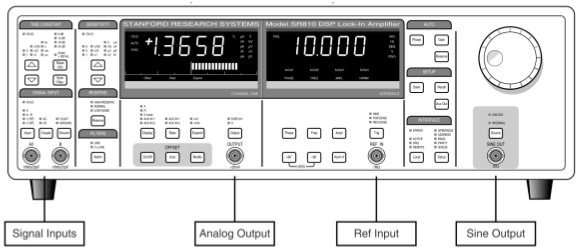
\includegraphics[width=\textwidth]{lock-in.png}
\caption{Front panel of the lock-in amplifier with the labeled components
\cite{ref:3}.}
\label{fig:7}
\end{figure*}
A Stanford Research Systems Model SR810 Lock-in amplifier is used in making the 
AC measurements in this experiment. The general layout of the front panel is 
shown on figure \ref{fig:7}. A lock-in amplifier is very useful in experiments 
that involve a lot of noisy data as it can reduce the noise from the data 
significantly and give a very clean signal. It can do so by multypling the 
input signal by the frequency of the reference signal and integrating it with 
respect to some time frame. The resulting DC signal has a frequency that is the 
same as that of the reference signal. The lock-in amplifier is very sensitive 
to different phases due to the orthogonality of sine and cosine functions 
\cite{ref:3}.
\\
For this experiment there will be a $V_{rms}$ output of 1.000 V that will pass 
through a 1 $M\Omega$ resistor to make a 1 $\mu A$ current signal. This signal 
will come from the Sine Output to a box with the resistor with two outputs that 
will connect to the wiring interface. The signal is received by the Signal 
Inputs. This will be an AC signal that will be transformed into a DC signal 
by the lock-in amplifier by the process described above. The following should 
be set to take measurements as well:
\begin{enumerate}[label=\alph*]
\item Couple to AC
\item Ground to Float
\item Time Constant to 1 s (1x1 s) and 12 dB
\item Display to R
\end{enumerate}
The sensitivity should be set to a value larger than that which you are trying 
to measure. It is recommended to use a sensitivity of 10 mV. Remember to hit 
the Phase button under AUTO on the right of the panel.
\subsection{DC source}
\begin{figure*}
\begin{minipage}{\textwidth}
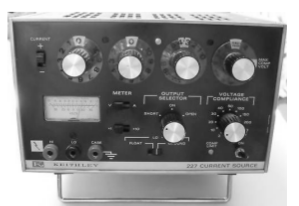
\includegraphics[width=\textwidth,height=3.5in]{DC-sourc.png}
\caption{Front panel of the DC \cite{ref:3}.}
\label{fig:8}
\end{minipage}
\end{figure*}
The DC source that is to be used is a Keithley 227 DC source. To perform the DC 
Hall Voltage measurements it will need to be set to output a 1 mA current. The 
knobs on the top of the device set the output current. Be mindful of where the 
light is as it is the decimal point. To produce a 1 mA current set the 
following to the said values \cite{ref:3}.
\begin{enumerate}[label=\alph*]
\item Set the units digit to 1 and all others to zero
\item Set the rightmost knob to mA with 300 MAX COMP VOLT
\end{enumerate}
Be sure to measure if the output is exactly 1 mA with a multi-meter. The first 
decimal knob may need to be played around with to get it as close to one as you 
can as it tends to be a bit loose and hard to set to exactly zero.
\subsection{Vacuum pumping system}
A single mechanical pump is used to vacuum both sections of the cryostat. 
Valves are provided on the respective spaces to give a good seal. When the pump 
is to be removed from the vacumming valves, make sure to close the valves to 
ensure that a vacuum is maintained at all times. If the pump is shut off 
before the valves are closed some air may be able to leak back into the 
vacuum spaces \cite{ref:3}.
\subsection{Electromagnet}
A water cooled electromagnet is used to produce the static magnetic field to 
make the Hall Effect measurements. There is a power supply unit that can be 
used to provide the current to the electromagnet. \textbf{Do not exceed 35 A 
on the power supply as it can overheat the magnet and permanently damage it}. 
To be able to measure two different magnetic field directions a bar is provided 
at the top of the sample probe. Refer to the markings on this bar to see the 
direction of the magnetic field with respect to the plane of the sample. 
\textbf{Make sure that the bar is well aligned with the magnetic plates prior 
to making measurements as we assume that the magnetic field is perfectly 
perpendicular to the sample. Tiny deviations from this could result in 
significant differences as the cross product in equation \ref{eqn:2} may not 
be perfect}. The table below shows the field strength in Tesla as a function 
of the electromagnet current.
\begin{minipage}{\linewidth}
\Centering
\begin{tabular}{|c|c|}
\hline
Current (A) & Magnetic Field (T) \\\hline
0 & 0 \\ \hline
5 & 0.1056 \\ \hline
10 & 0.2125 \\ \hline
15 & 0.3179 \\ \hline
20 & 0.4265 \\ \hline
25 & 0.5258 \\ \hline
30 & 0.6058 \\ \hline
35 & 0.6678 \\ \hline
\end{tabular}
\captionof{table}{Magnetic field strength as a function of current. Measured 
experimentally \cite{ref:3}.}
\label{tbl:2}
\end{minipage}
When plotted this looks like the plot on the figure below.
\center
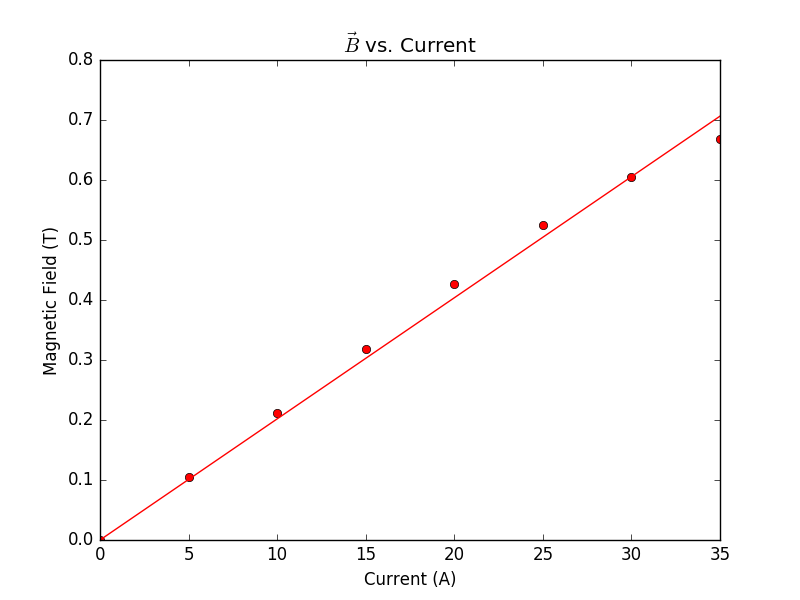
\includegraphics[width=\linewidth]{magnetic-field-vs-current.png}
\justify
\section{Results and Discussion}
\begin{figure*}
\begin{minipage}{\textwidth}
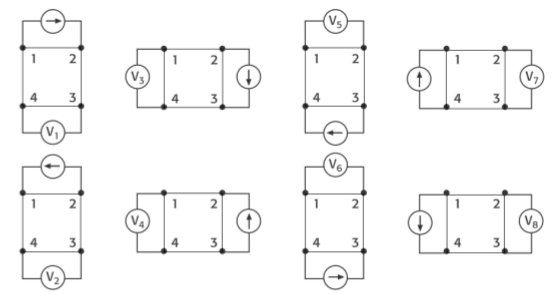
\includegraphics[width=\linewidth]{four-contact.png}
\caption{All 8 configurations for part ii in the experiment \cite{ref:3}}
\label{fig:9}
\end{minipage}
\vfill
\begin{minipage}{0.46\textwidth}
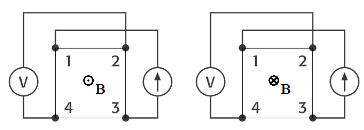
\includegraphics[width=\linewidth]{room-temp-config.png}
\caption{DC Hall measurement configuration for the room temperature measurement 
in part iii of the experiment \cite{ref:3}.}
\label{fig:10}
\end{minipage}
\hfill
\begin{minipage}{0.46\textwidth}
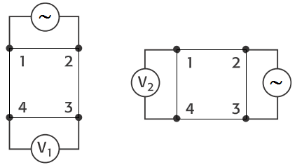
\includegraphics[width=\linewidth]{res-temp-config.png}
\caption{AC resistivity measurement configurations for part v of the experiment 
\cite{ref:3}.}
\label{fig:11}
\end{minipage}
\vfill
\begin{minipage}{\textwidth}
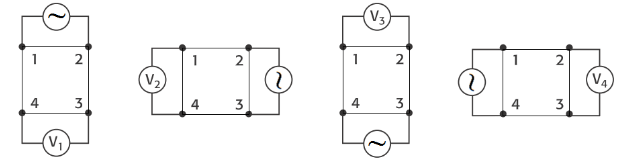
\includegraphics[width=\linewidth]{AC-4-contact.png}
\caption{AC resistivity measurement configurations for part iv in the 
experiment \cite{ref:3}.}
\label{fig:12}
\end{minipage}
\end{figure*}
All of the longitudal directions will be using the labeling as shown on figure 
\ref{fig:9}.
\subsection{DC 2-contact resistance}
In this part of the experiment we measured the resistance of the sample using 
an ohm-meter for the four possible longitudal directions.
\\
The data that is gotten is shown below.
\begin{minipage}{\linewidth}
\Centering
\begin{tabular}{|c|c|}
\hline
Direction & Resistance ($k\Omega$) \\ \hline
1,2 & 4.77 \\ \hline
2,3 & 2.57 \\ \hline
3,4 & 6.62 \\ \hline
4,1 & 7.02 \\ \hline
\end{tabular}
\captionof{table}{Data for part (i)}
\label{tbl:3}
\end{minipage}
From this data it is not possible to calculate the resistivity as we have a 
the resistance of the sample through those points and according to equation 
\ref{eqn:6} we need to know the other dimensions of the sample, for which, we 
did not.
\subsection{DC 4-contact resistance}
In this portion of the experiment we measured the voltage from passing current 
through two adjacent points and measuring the voltage through the other two. 
All 8 configurations that are used are shown on figure \ref{fig:9}. 
The data for it is shown on the table below where the direction of the current 
flow is important as it is we are the DC source. The current value was set to 
be 0.99 mA.
\begin{minipage}{\linewidth}
\Centering
\begin{tabular}{|c|c|}
\hline
Direction & Absolute \\ From $\to\,$ to & Voltage (mV) \\ \hline
1 $\to\,$ 2 & 1.169 \\ \hline
2 $\to\,$ 1 & 1.179 \\ \hline
2 $\to\,$ 3 & 0.3037 \\ \hline
3 $\to\,$ 2 & 0.2955 \\ \hline
3 $\to\,$ 4 & 1.069 \\ \hline
4 $\to\,$ 3 & 0.839 \\ \hline
4 $\to\,$ 1 & 0.3003 \\ \hline
4 $\to\,$ 1 & 0.2821 \\ \hline
\end{tabular}
\captionof{table}{Flow of current and measured voltage for DC 4-contact 
resistance.}
\label{tbl:4}
\end{minipage}
From these values the van der Pauw method can be applied to calculate the 
resistivity of the sample. Since the value of the measured voltage is expected 
to be the same in both directions (ie. from A to B and B to A), the average of 
the two values was taken and used in the calculations. The van der Pauw 
resistivity was calculated using equations \ref{eqn:7} and \ref{eqn:9} using 
C++. The results are shown in the following table where the current direction 
is no longer important.
\begin{minipage}{\linewidth}
\Centering
\begin{tabular}{|c|c|}
\hline
Direction & Resistivity ($\Omega m$) \\ \hline
1,2 & 0.877 $\pm$ 0.004 \\ \hline
2,3 & 0.774 $\pm$ 0.004 \\ \hline
3,4 & 0.764 $\pm$ 0.004 \\ \hline
4,1 & 0.867 $\pm$ 0.004 \\ \hline
\end{tabular}
\captionof{table}{Results of the resistivity calculations using the van der 
Pauw method for the DC 4-contact resistance.}
\label{tbl:5}
\end{minipage}
For the error analysis a constant error of 0.010 mV was assumed for all of the 
measurements and the error in the f value was ignored.
\subsection{DC Hall Effect measurement - determining carrier type}
\begin{figure*}
\begin{minipage}[t]{0.46\textwidth}
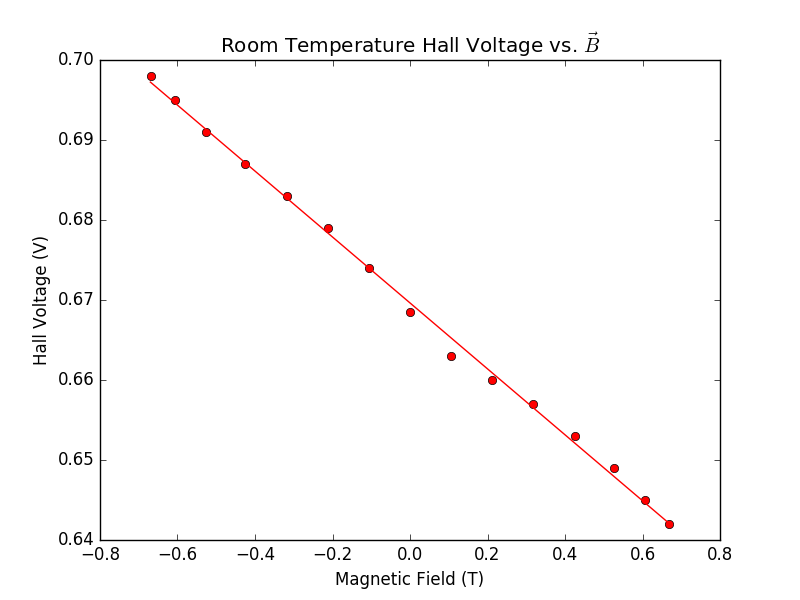
\includegraphics[width=\linewidth]{room-temperature-dc.png}
\caption{DC Room temperature Hall Voltage measurements as a function of 
magnetic field. A linear fit line is provided in the table with a slope of 
-0.0412 $\pm$ 0.0005 and a y intercept of 0.6696 $\pm$ 0.0002.}
\label{fig:13}
\end{minipage}
\hfill
\begin{minipage}[t]{0.46\textwidth}
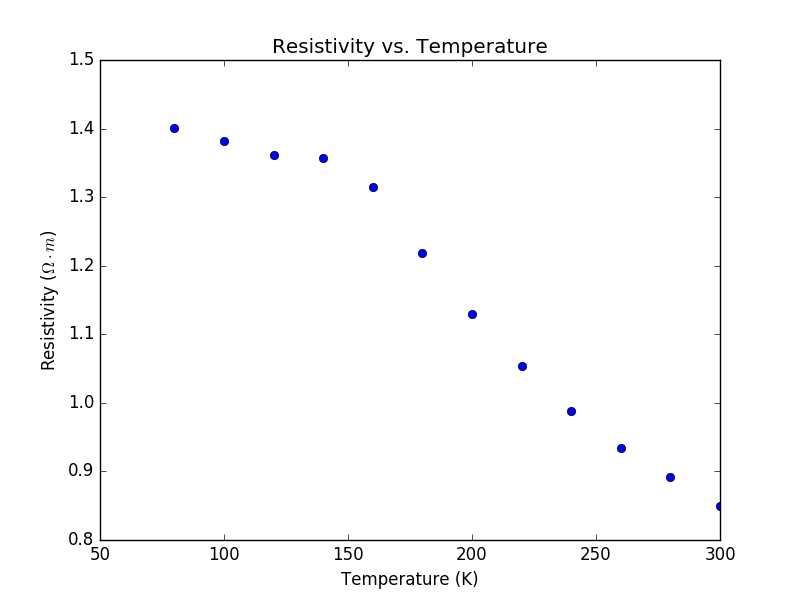
\includegraphics[width=\linewidth]{resistivity-vs-temp.png}
\caption{Plot of resistivity as a function of temperature. Resistivity 
calculated with the van der Pauw method.}
\label{fig:14}
\end{minipage}
\end{figure*}
For this part of the experiment the carrier type was determing by analyzing the 
slope of the line of data that was taken at different magnetic field values 
taken at room temperature. The configurations used are the ones showed on 
figure \ref{fig:10}. A current value of 1.00 mA was passed through the 
sample. The data is shown below.
\begin{minipage}{\linewidth}
\Centering
\begin{tabular}{|c|c|}
\hline
Magnetic Field (T) & $V_{Hall}$ (V) \\ \hline
-0.6678 & 0.698 \\ \hline
-0.6058 & 0.695 \\ \hline
-0.5258 & 0.691 \\ \hline
-0.4265 & 0.687 \\ \hline
-0.3179 & 0.683 \\ \hline
-0.2125 & 0.679 \\ \hline
-0.1056 & 0.674 \\ \hline
0.0000 & 0.6685 \\ \hline
0.1056 & 0.663 \\ \hline
0.2125 & 0.660 \\ \hline
0.3179 & 0.657 \\ \hline
0.4265 & 0.653 \\ \hline
0.5258 & 0.649 \\ \hline
0.6058 & 0.645 \\ \hline
0.6678 & 0.642 \\ \hline
\end{tabular}
\captionof{table}{Data from measuring the Hall Voltage using a DC source.}
\label{tbl:6}
\end{minipage}
When the data from table \ref{tbl:6} is plotted we get the plot shown on figure 
\ref{fig:13}. A linear fir was applied to see that there is a very linear trend 
in the Hall Voltage as a function if the magnetic field.
\\
In order, to identify the type of carriers that are present in the 
semiconductor sample it is helpful to go back to equations \ref{eqn:15} and 
\ref{eqn:16}, both of which, were set up in a very clever way to show that the 
sign of the slope is equal to the sign of the charge carriers. This comes about 
because, looking at equation \ref{eqn:15} it was said that if the Hall constant 
is negative then we have negatively charged carriers. Which, we do as per the 
slope of the line that is given in the caption of figure \ref{fig:13} for which 
equation \ref{eqn:15} can be re-written in the following way. 
\begin{equation}
R_{H} = s\frac{t}{I}
\label{eqn:18}
\end{equation}
Where, t and I are both positive and s is the slope from the data on table 
\ref{tbl:6} and can be positive or negative.
\\
In conclusion, 
the semiconductor sample is a n-type semiconductor with excess electrons.
\subsection{AC 4-contact resistance}
For this part of the experiment much like in part ii we are interested in 
finding the resistivity of the sample by measuring voltages through adjacent 
points on the sample and using the van der Pauw method on the data. The 
configurations that were used are shown in figure \ref{fig:12}. The data shown 
below was taken in the order of the configurations.
\begin{minipage}{\linewidth}
\Centering
\begin{tabular}{|c|c|}
\hline
Direction & Voltage (mV) \\ \hline
1,2 & 1.045 \\ \hline
2,3 & 0.313 \\ \hline
3,4 & 0.733 \\ \hline
4,1 & 0.312 \\ \hline
\end{tabular}
\captionof{table}{Data from the measurement of the voltage by passing a AC 
source from the Lock-in amplifier.}
\label{tbl:7}
\end{minipage}
When the van der Pauw method was applied to the data on table \ref{tbl:7} we 
got the following resistivities.
\begin{minipage}{\linewidth}
\Centering
\begin{tabular}{|c|c|}
\hline
Direction & Resistivity ($\Omega m$) \\ \hline
1,2 & 0.823 $\pm$ 0.004 \\ \hline
2,3 & 0.670 $\pm$ 0.004 \\ \hline
3,4 & 0.669 $\pm$ 0.004 \\ \hline
4,1 & 0.822 $\pm$ 0.004 \\ \hline
\end{tabular}
\captionof{table}{Results from applying the van der Pauw method on the data 
from table \ref{tbl:7}.}
\label{tbl:8}
\end{minipage}
Where, we also assume the error in measurement to be 0.005 mV anf the f value 
to contribute an ignorable portion.
\\
When comparing the two data sets from tables \ref{tbl:5} and \ref{tbl:8} we see 
that the results do differ and are not equal to each other within their 
uncertainties. We believe this to be because in the DC measurement there may 
have been noise from other sources which do not get cancelled and can 
contribute to a greater error degree. Also, the slight magnetization in the 
metallic plates of the electromagnet may skew the results by inducing a slight 
Hall voltage.
\\
We believe that the AC measurements of the resistivities are more accurate than 
the DC due to noise from other DC sources that may arise in the sample.
\subsection{Resistivity versus Temperature}
For this part of the experiment we wanted to find the relation between 
resistivity of the sample and the temperature. The configurations that were used to 
take the data were those shown of figure \ref{fig:11}. The data that we took 
is shown in the table below. Where the first row gives through which points 
the current is being sent through and the second begins the data column labels.
\begin{minipage}{\linewidth}
\Centering
\begin{tabular}{|c|c|c|}
\hline
Flow of  & Through & Thorugh \\ current & 1,2 & 3,4 \\ \hline \hline
Temperature (K) & Voltage (mv) & Voltage (mV) \\ \hline
79.88 & 1.870 & 0.493 \\ \hline
100.00 & 1.838 & 0.489 \\ \hline
120.04 & 1.796 & 0.488 \\ \hline
140.04 & 1.766 & 0.497 \\ \hline
160.04 & 1.705 & 0.484 \\ \hline
180.04 & 1.574 & 0.452 \\ \hline
200.01 & 1.451 & 0.422 \\ \hline
220.1 & 1.338 & 0.400 \\ \hline
240.1 & 1.244 & 0.381 \\ \hline
260.1 & 1.164 & 0.365 \\ \hline
280.0 & 1.276 & 0.280 \\ \hline
300.0 & 1.186 & 0.278 \\ \hline
\end{tabular}
\captionof{table}{Voltage data taken at various temperatures with an AC source from 
the Lock-in amplifier. Should be noted that the last two measurements for 280K 
and 300K were taken on a different day so this may account for the sharp change 
in the data.}
\label{tbl:9}
\end{minipage}
Much like we have been doing in the previous parts of the experiment we use the 
van der Pauw method to get the resistivities at the various temperatures. When 
we do this we get the following data.
\begin{minipage}{\linewidth}
\Centering
\begin{tabular}{|c|c|}
\hline
Temp.(K) & Resistivity ($\Omega m$) \\ \hline
79.88 & 1.40 $\pm$ 0.01 \\ \hline
100.00 & 1.38 $\pm$ 0.01 \\ \hline
120.04 & 1.36 $\pm$ 0.01 \\ \hline
140.04 & 1.36 $\pm$ 0.01 \\ \hline
160.04 & 1.31 $\pm$ 0.01 \\ \hline
180.04 & 1.22 $\pm$ 0.01 \\ \hline
200.01 & 1.13 $\pm$ 0.01 \\ \hline
220.1 & 1.05 $\pm$ 0.01 \\ \hline
240.1 & 0.99 $\pm$ 0.01 \\ \hline
260.1 & 0.93 $\pm$ 0.01 \\ \hline
280.0 & 0.89 $\pm$ 0.01 \\ \hline
300.0 & 0.85 $\pm$ 0.01 \\ \hline
\end{tabular}
\captionof{table}{Results of using the van der Pauw method on the data from table \ref{tbl:9}.}
\label{tbl:10}
\end{minipage}
We assumed errors in our data to be 0.010 mV and the contribution from the f 
value error once again to be insignificant.
\\
The data from table \ref{tbl:10} is plotted on figure \ref{fig:14}. Now the 
interesting thing about the plot is the slight plateau at the very beginning 
of the plot. This goes against what we are initially taught in electrodynamics, 
in which, the resistivity of a material goes up with increasing temperature. 
While that holds for most materials the same does not necessarily apply for 
semiconductors. The reason being, band gap energy. In semiconductors there is a 
certain band gap which is related to the spacings between orbital shells of 
the atom. So we also know that temperature can be represented as vibrational 
kinetic energy. So what does this all mean? In semiconductors there are two 
different shell levels: the valence and the conduction. Where the valence is 
the highest occupied shell by electrons and the conduction includes the 
excitation levels of electrons. At extremely low temperatures the electrons 
have a relatively low vibrational kinetic energy and from the Fermi-Dirac 
statistics formula.
\begin{equation}
f(E) = \frac{1}{\exp{(E-E_{F})/kT)}+1}
\label{eqn:18}
\end{equation}
Where, k is the boltzmann constant, E is the energy at which we are looking 
for the electron, $E_{F}$ is the fermi energy and T is the temperature. We see 
that as T aproaches 0 and we are below the fermi level the probability of 
finding an electron in the valence band is 1 and 0 for the conduction band. As the 
temperature increases the function shifts from being a rigid step-function and 
smooths out at the ends until the probability of electrons in the conduction 
band is non-zero and there can be conduction of electrons and as the 
temperature increases the number of electrons that can be found on the 
conduction band decreases. Therefore, the resistivity decreases with 
temperature sice there will be more electrons readily available to conduct 
electricity.
\\
The reason why it may plateau at a certain value may be due to the fact that 
the semiconductor is an n-type silicon sample, so not all of the electrons will 
be able to go to 
the valence band at low temperatures so some stay in the conduction band but 
this number is very small to those that are found in the valence.
\subsection{AC Hall Voltage}
\begin{figure*}
\begin{minipage}{\textwidth}
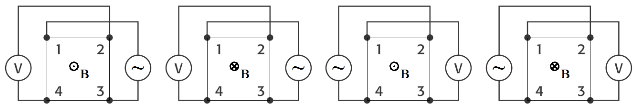
\includegraphics[width=0.6\linewidth,height=0.5in]{hall-config.png}
\caption{AC Hall Effect measurement configurations labeling for the data was 
cofiguration 1-4 from left to right \cite{ref:3}}
\label{fig:15}
\end{minipage}
\vfill
\begin{minipage}[t]{0.46\textwidth}
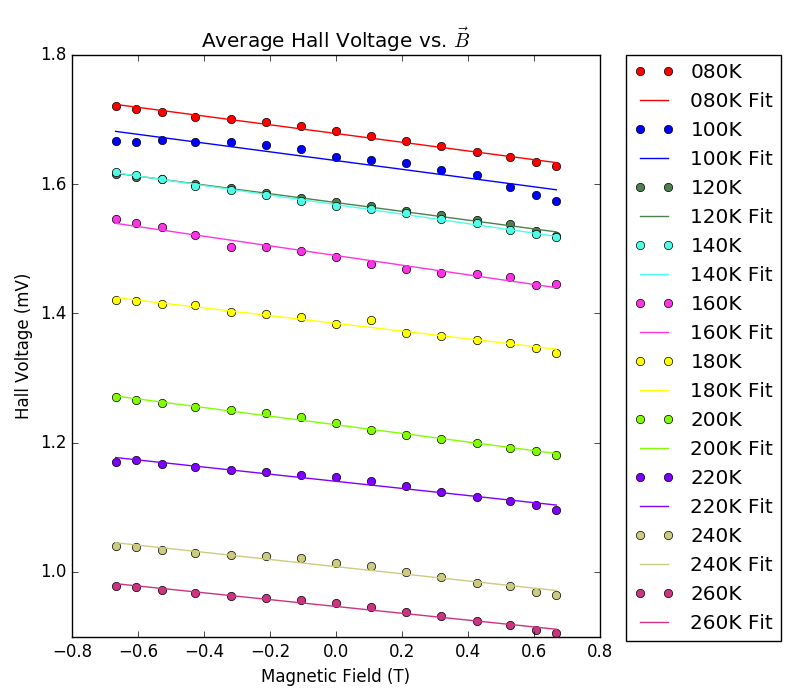
\includegraphics[width=\linewidth]{average-hall-volt.png}
\caption{Plot of average Hall Voltages as a function of magnetic field. Refer
to the legend to navigate through the different temperature values.}
\label{fig:16}
\end{minipage}
\hfill
\begin{minipage}[t]{0.46\textwidth}
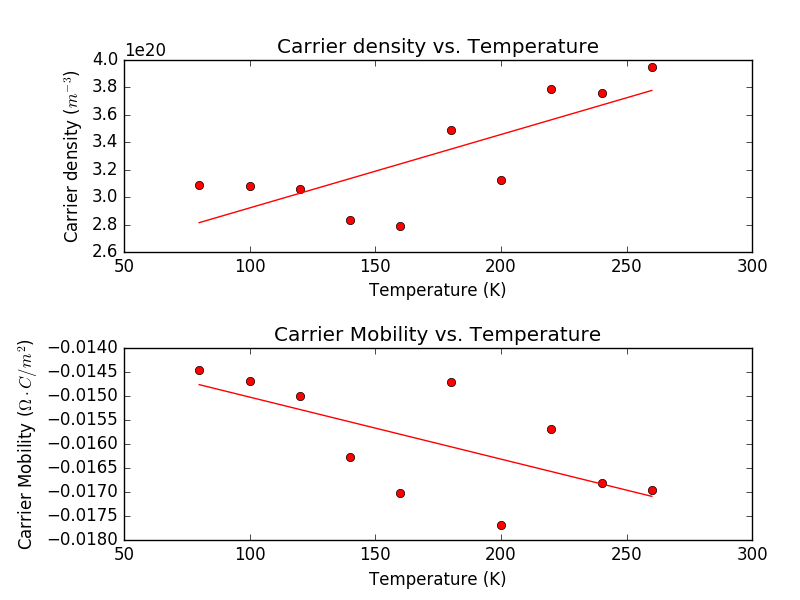
\includegraphics[width=\linewidth]{carrier-mobility-density.png}
\caption{Plot of the Carrier density and mobility calculated from the slopes of 
figure \ref{fig:16}. The fit lines are only trend lines intended to help 
see the general trend of the data.}
\label{fig:17}
\end{minipage}
\end{figure*}
In this final section of the experiment we found the Hall Voltages for 
different temperatures at different magnetic field strengths. The data that was 
taken for this part of the experiment will be included in the next section due 
to the amount of it. The data on figure \ref{fig:16} was fitted linearly with 
the equation y = ax + b. The data used was the average of the two 
configurations shown on \ref{fig:15}. The parameter values of the fit are 
displayed on the 
table below. We only took data from 80 to 260 K.
\begin{minipage}{\linewidth}
\Centering
\begin{tabular}{|c|c|c|}
\hline
Fit-line & Parameter & Parameter \\ Temp. (K) & a & b \\ \hline
80 & -0.067 $\pm$ 0.002 & 1.6784 $\pm$ 0.0009 \\ \hline 
100 & -0.068 $\pm$ 0.006 & 1.637 $\pm$ 0.003 \\ \hline 
120 & -0.068 $\pm$ 0.001 & 1.5716 $\pm$ 0.0007 \\ \hline 
140 & -0.074 $\pm$ 0.001 & 1.5684 $\pm$ 0.0005 \\ \hline 
160 & -0.075 $\pm$ 0.003 & 1.490 $\pm$ 0.001 \\ \hline 
180 & -0.060 $\pm$ 0.002 & 1.385 $\pm$ 0.001 \\ \hline 
200 & -0.067 $\pm$ 0.001 & 1.2277 $\pm$ 0.0006 \\ \hline 
220 & -0.055 $\pm$ 0.003 & 1.140 $\pm$ 0.001 \\ \hline 
240 & -0.055 $\pm$ 0.003 & 1.008 $\pm$ 0.001 \\ \hline 
260 & -0.053 $\pm$ 0.002 & 0.9466 $\pm$ 0.0009 \\ \hline 
\end{tabular}
\captionof{table}{Slopes and intercepts of the data in figure \ref{fig:16}}
\label{tbl:11}
\end{minipage}
With the slopes that are shown abpove we were then able to use equations 
\ref{eqn:16} and \ref{eqn:17} replacing V/B with the slope to calculate the 
carrier density and mobility. For the error in both we used simple error 
propagation in the slope to calculate the respective uncertanties. Both the 
fits and the calculations for this part were done solely in python.
The data 
that we calculated then is shown below.
\begin{minipage}{\linewidth}
\Centering
\begin{tabular}{|c|c|c|}
\hline
Temp.(K) & Density & Mobility 
\\ & ($\times10^{20}m^{-3}$) & ($\times10^{-2}\Omega C / m^2$) \\ \hline
80 & 3.08 $\pm$ 0.09 & 1.44 $\pm$ 0.05 \\ \hline
100 & 3.1 $\pm$ 0.3 & 1.50 $\pm$ 0.05 \\ \hline
120 & 3.06 $\pm$ 0.07 & 1.50 $\pm$ 0.03 \\ \hline
140 & 2.83 $\pm$ 0.04 & 1.63 $\pm$ 0.03 \\ \hline
160 & 2.8 $\pm$ 0.1 & 1.70 $\pm$ 0.07 \\ \hline
180 & 3.5 $\pm$ 0.1 & 1.47 $\pm$ 0.06 \\ \hline
200 & 3.12 $\pm$ 0.07 & 1.77 $\pm$ 0.04 \\ \hline
220 & 3.8 $\pm$ 0.2 & 1.57 $\pm$ 0.07 \\ \hline
240 & 3.8 $\pm$ 0.2 & 1.68$\pm$ 0.09 \\ \hline
260 & 3.9 $\pm$ 0.2 & 1.70 $\pm$ 0.07 \\ \hline
\end{tabular}
\captionof{table}{Results of the carrier density and mobility using the 
slopes from table \ref{tbl:11}}
\label{tbl:12}
\end{minipage}
The data on table \ref{tbl:12} is plotted on figure \ref{fig:17}. The plots do 
not look like they should and we believe that this was due to the equipment 
since most of our time in lab was spent troubleshooting the cause of large 
errors and fluctuations in the received values of the voltage into the 
Lock-in amplifier. However, when fitted with a general trend line it follows 
the expected behaviors that both should folllow an inverse trend to that seen 
in figure \ref{fig:14}. So there should be a slight plateau at low temperatures 
and then it rises as the temperature goes up. From the explanation given for 
the resistivity decrease the carrier density is an increasing function.
\subsection{Data for part vi}
Here is all of the data from part iv which is arranged into three columns: 
Magnetic field, configurations 1,2 and configurations 3,4. Arranged in 
increasing temperature. Something to notice is that the third column has a 
positive slope where the 2 is negative when the data was plotted the magnetic 
field of the third column was negated to get a negative slope. This is due to 
the flow direction of the current and the definition of our axes were inverted. 
However, the data will be presented as it was taken.
\begin{minipage}{\linewidth}
\Centering
Temperature = 80 K
\begin{tabular}{|c|c|c|}
\hline
Magnetic Field (T) & V\textsubscript{1,2} (mV) & V\textsubscript{3,4} (mV) \\ \hline
-0.6678 & 1.730 & 1.620 \\ \hline
-0.6058 & 1.726 & 1.626 \\ \hline
-0.5258 & 1.720 & 1.635 \\ \hline
-0.4265 & 1.712 & 1.641 \\ \hline
-0.3179 & 1.708 & 1.650 \\ \hline
-0.2125 & 1.703 & 1.660 \\ \hline
-0.1056 & 1.698 & 1.667 \\ \hline
0.0000 & 1.691 & 1.674 \\ \hline
0.1056 & 1.683 & 1.683 \\ \hline
0.2125 & 1.675 & 1.688 \\ \hline
0.3179 & 1.667 & 1.693 \\ \hline
0.4265 & 1.657 & 1.697 \\ \hline
0.5258 & 1.650 & 1.702 \\ \hline
0.6058 & 1.642 & 1.707 \\ \hline
0.6678 & 1.635 & 1.711 \\ \hline
\end{tabular}
\end{minipage}
\begin{minipage}{\linewidth}
\Centering
Temperature = 100 K
\begin{tabular}{|c|c|c|}
\hline
Magnetic Field (T) & V\textsubscript{1,2} (mV) & V\textsubscript{3,4} (mV) \\ \hline
-0.6678 & 1.671 & 1.567 \\ \hline
-0.6058 & 1.667 & 1.575 \\ \hline
-0.5258 & 1.675 & 1.592 \\ \hline
-0.4265 & 1.678 & 1.609 \\ \hline
-0.3179 & 1.671 & 1.617 \\ \hline
-0.2125 & 1.667 & 1.626 \\ \hline
-0.1056 & 1.662 & 1.631 \\ \hline
0.0000 & 1.647 & 1.638 \\ \hline
0.1056 & 1.644 & 1.646 \\ \hline
0.2125 & 1.638 & 1.655 \\ \hline
0.3179 & 1.628 & 1.659 \\ \hline
0.4265 & 1.620 & 1.653 \\ \hline
0.5258 & 1.599 & 1.663 \\ \hline
0.6058 & 1.591 & 1.663 \\ \hline
0.6678 & 1.581 & 1.662 \\ \hline
\end{tabular}
\end{minipage}
\begin{minipage}{\linewidth}
\Centering
Temperature = 120 K
\begin{tabular}{|c|c|c|}
\hline
Magnetic Field (T) & V\textsubscript{1,2} (mV) & V\textsubscript{3,4} (mV) \\ \hline
-0.6678 & 1.621 & 1.514 \\ \hline
-0.6058 & 1.616 & 1.521 \\ \hline
-0.5258 & 1.614 & 1.531 \\ \hline
-0.4265 & 1.607 & 1.540 \\ \hline
-0.3179 & 1.600 & 1.548 \\ \hline
-0.2125 & 1.592 & 1.553 \\ \hline
-0.1056 & 1.586 & 1.560 \\ \hline
0.0000 & 1.578 & 1.566 \\ \hline
0.1056 & 1.573 & 1.572 \\ \hline
0.2125 & 1.564 & 1.580 \\ \hline
0.3179 & 1.558 & 1.588 \\ \hline
0.4265 & 1.550 & 1.595 \\ \hline
0.5258 & 1.545 & 1.601 \\ \hline
0.6058 & 1.534 & 1.605 \\ \hline
0.6678 & 1.526 & 1.609 \\ \hline
\end{tabular}
\end{minipage}
\begin{minipage}{\linewidth}
\Centering
Temperature = 140 K
\begin{tabular}{|c|c|c|}
\hline
Magnetic Field (T) & V\textsubscript{1,2} (mV) & V\textsubscript{3,4} (mV) \\ \hline
-0.6678 & 1.637 & 1.521 \\ \hline
-0.6058 & 1.630 & 1.526 \\ \hline
-0.5258 & 1.623 & 1.534 \\ \hline
-0.4265 & 1.612 & 1.544 \\ \hline
-0.3179 & 1.608 & 1.550 \\ \hline
-0.2125 & 1.600 & 1.562 \\ \hline
-0.1056 & 1.592 & 1.567 \\ \hline
0.0000 & 1.574 & 1.559 \\ \hline
0.1056 & 1.557 & 1.557 \\ \hline
0.2125 & 1.549 & 1.568 \\ \hline
0.3179 & 1.542 & 1.575 \\ \hline
0.4265 & 1.535 & 1.581 \\ \hline
0.5258 & 1.525 & 1.592 \\ \hline
0.6058 & 1.519 & 1.599 \\ \hline
0.6678 & 1.514 & 1.600 \\ \hline
\end{tabular}
\end{minipage}
\begin{minipage}{\linewidth}
\Centering
Temperature = 160 K
\begin{tabular}{|c|c|c|}
\hline
Magnetic Field (T) & V\textsubscript{1,2} (mV) & V\textsubscript{3,4} (mV) \\ \hline
-0.6678 & 1.556 & 1.447 \\ \hline
-0.6058 & 1.552 & 1.453 \\ \hline
-0.5258 & 1.544 & 1.456 \\ \hline
-0.4265 & 1.529 & 1.462 \\ \hline
-0.3179 & 1.516 & 1.470 \\ \hline
-0.2125 & 1.511 & 1.476 \\ \hline
-0.1056 & 1.505 & 1.482 \\ \hline
0.0000 & 1.493 & 1.482 \\ \hline
0.1056 & 1.471 & 1.488 \\ \hline
0.2125 & 1.461 & 1.494 \\ \hline
0.3179 & 1.455 & 1.490 \\ \hline
0.4265 & 1.460 & 1.513 \\ \hline
0.5258 & 1.456 & 1.523 \\ \hline
0.6058 & 1.436 & 1.528 \\ \hline
0.6678 & 1.444 & 1.535 \\ \hline
\end{tabular}
\end{minipage}
\begin{minipage}{\linewidth}
\Centering
Temperature = 180 K
\begin{tabular}{|c|c|c|}
\hline
Magnetic Field (T) & V\textsubscript{1,2} (mV) & V\textsubscript{3,4} (mV) \\ \hline
-0.6678 & 1.426 & 1.333 \\ \hline
-0.6058 & 1.420 & 1.344 \\ \hline
-0.5258 & 1.415 & 1.347 \\ \hline
-0.4265 & 1.405 & 1.350 \\ \hline
-0.3179 & 1.396 & 1.358 \\ \hline
-0.2125 & 1.393 & 1.364 \\ \hline
-0.1056 & 1.390 & 1.369 \\ \hline
0.0000 & 1.388 & 1.378 \\ \hline
0.1056 & 1.410 & 1.398 \\ \hline
0.2125 & 1.375 & 1.404 \\ \hline
0.3179 & 1.373 & 1.409 \\ \hline
0.4265 & 1.367 & 1.420 \\ \hline
0.5258 & 1.363 & 1.415 \\ \hline
0.6058 & 1.350 & 1.417 \\ \hline
0.6678 & 1.346 & 1.416 \\ \hline
\end{tabular}
\end{minipage}
\begin{minipage}{\linewidth}
\Centering
Temperature = 200 K
\begin{tabular}{|c|c|c|}
\hline
Magnetic Field (T) & V\textsubscript{1,2} (mV) & V\textsubscript{3,4} (mV) \\ \hline
-0.6678 & 1.279 & 1.187 \\ \hline
-0.6058 & 1.273 & 1.193 \\ \hline
-0.5258 & 1.268 & 1.198 \\ \hline
-0.4265 & 1.263 & 1.203 \\ \hline
-0.3179 & 1.261 & 1.209 \\ \hline
-0.2125 & 1.256 & 1.217 \\ \hline
-0.1056 & 1.251 & 1.221 \\ \hline
0.0000 & 1.234 & 1.226 \\ \hline
0.1056 & 1.219 & 1.230 \\ \hline
0.2125 & 1.207 & 1.236 \\ \hline
0.3179 & 1.202 & 1.240 \\ \hline
0.4265 & 1.195 & 1.246 \\ \hline
0.5258 & 1.186 & 1.254 \\ \hline
0.6058 & 1.182 & 1.258 \\ \hline
0.6678 & 1.176 & 1.262 \\ \hline
\end{tabular}
\end{minipage}
\begin{minipage}{\linewidth}
\Centering
Temperature = 220 K
\begin{tabular}{|c|c|c|}
\hline
Magnetic Field (T) & V\textsubscript{1,2} (mV) & V\textsubscript{3,4} (mV) \\ \hline
-0.6678 & 1.172 & 1.096 \\ \hline
-0.6058 & 1.174 & 1.100 \\ \hline
-0.5258 & 1.169 & 1.107 \\ \hline
-0.4265 & 1.164 & 1.114 \\ \hline
-0.3179 & 1.161 & 1.122 \\ \hline
-0.2125 & 1.156 & 1.130 \\ \hline
-0.1056 & 1.154 & 1.139 \\ \hline
0.0000 & 1.150 & 1.144 \\ \hline
0.1056 & 1.141 & 1.146 \\ \hline
0.2125 & 1.135 & 1.152 \\ \hline
0.3179 & 1.126 & 1.156 \\ \hline
0.4265 & 1.119 & 1.162 \\ \hline
0.5258 & 1.112 & 1.164 \\ \hline
0.6058 & 1.107 & 1.171 \\ \hline
0.6678 & 1.097 & 1.168 \\ \hline
\end{tabular}
\end{minipage}
\begin{minipage}{\linewidth}
\Centering
Temperature = 240 K
\begin{tabular}{|c|c|c|}
\hline
Magnetic Field (T) & V\textsubscript{1,2} (mV) & V\textsubscript{3,4} (mV) \\ \hline
-0.6678 & 1.041 & 0.963 \\ \hline
-0.6058 & 1.038 & 0.968 \\ \hline
-0.5258 & 1.035 & 0.977 \\ \hline
-0.4265 & 1.029 & 0.983 \\ \hline
-0.3179 & 1.028 & 0.992 \\ \hline
-0.2125 & 1.024 & 0.997 \\ \hline
-0.1056 & 1.022 & 1.008 \\ \hline
0.0000 & 1.015 & 1.014 \\ \hline
0.1056 & 1.011 & 1.020 \\ \hline
0.2125 & 1.002 & 1.025 \\ \hline
0.3179 & 0.993 & 1.024 \\ \hline
0.4265 & 0.984 & 1.029 \\ \hline
0.5258 & 0.979 & 1.033 \\ \hline
0.6058 & 0.971 & 1.038 \\ \hline
0.6678 & 0.965 & 1.039 \\ \hline
\end{tabular}
\end{minipage}
\begin{minipage}{\linewidth}
\Centering
Temperature = 260 K
\begin{tabular}{|c|c|c|}
\hline
Magnetic Field (T) & V\textsubscript{1,2} (mV) & V\textsubscript{3,4} (mV) \\ \hline
-0.6678 & 0.979 & 0.906 \\ \hline
-0.6058 & 0.976 & 0.910 \\ \hline
-0.5258 & 0.972 & 0.917 \\ \hline
-0.4265 & 0.968 & 0.923 \\ \hline
-0.3179 & 0.965 & 0.931 \\ \hline
-0.2125 & 0.961 & 0.937 \\ \hline
-0.1056 & 0.958 & 0.945 \\ \hline
0.0000 & 0.952 & 0.951 \\ \hline
0.1056 & 0.946 & 0.955 \\ \hline
0.2125 & 0.939 & 0.959 \\ \hline
0.3179 & 0.932 & 0.962 \\ \hline
0.4265 & 0.926 & 0.968 \\ \hline
0.5258 & 0.919 & 0.971 \\ \hline
0.6058 & 0.911 & 0.976 \\ \hline
0.6678 & 0.906 & 0.978 \\ \hline
\end{tabular}
\end{minipage}
\section{Conclusion}
We were able to find all that we were looking for and found what we expected with the 
temperature dependence of the carrier mobility and density along with the 
resistivity. The Hall Effect has been a method that has been very helpful in 
the study of materials by allowing us to gain more knowledge about what it is 
that actually moves the electricity and how temperature affects it. 
//
After the birth of quantum mechanics the Hall Effect became more easily 
explained since the electron and other sub-atomic particles were coming to 
light and it allowed scientists to add to it. One of the advancements is the 
Quantum Hall Effect (QHE) from which cam Fractional QHE and Integral QHE with 
the same goal to gain a deeper understanding of the materials that we work with 
and interact with on our day to day lives \cite{ref:6}.
\begin{thebibliography}{9}
\bibitem{ref:1}
Purcell, E. M.; Morin, D. J. (2013). Electricity and Magnetism. New York: 
\emph{Cambridge University Press}, 314-317.
\bibitem{ref:2}
(2016,December 24).Van der Pauw method. \emph{Wikipedia}. 
https://en.wikipedia.org/wiki/\\Van\_der\_Pauw\_method
\bibitem{ref:3}
UB 2015 Lab Manual. Hall Effect
\bibitem{ref:4}
Van der Pauw, L. J. (1958). A method of measuring specific resistivity and 
Hall Effect of discs of arbitrary shape. \emph{Philips Research reports, 13}, 
1-9.
\bibitem{ref:5}
LakeShore (2000). User's Manual Model 330 Autotuning Temperature Controller.
\bibitem{ref:6}
Lynn, J. W. (1990). The Quantum Hall Effect. 175 Fifth Avenue, New York, 
New York: \emph{Springer-Verlag New York}.
\end{thebibliography}
\end{document}
